
%(BEGIN_QUESTION)
% Copyright 2009, Tony R. Kuphaldt, released under the Creative Commons Attribution License (v 1.0)
% This means you may do almost anything with this work of mine, so long as you give me proper credit

This chlorination control system adds chlorine to a wastewater stream to disinfect it before discharging to a natural body of water.  Two chlorine valves of vastly different size exist to throttle the flow of chlorine to the water: a small valve intended for low-flow operation, and a large valve that opens up when high flow is needed.  A residual chlorine analyzer outputs 4 mA with no chlorine in the water and 20 mA with high levels of chlorine in the water:
 
$$\includegraphics[width=15.5cm]{i03783x01.eps}$$

Assuming direct action in the controller, determine the proper split ranges of the two control valves:

% No blank lines allowed between lines of an \halign structure!
% I use comments (%) instead, so that TeX doesn't choke.

$$\vbox{\offinterlineskip
\halign{\strut
\vrule \quad\hfil # \ \hfil & 
\vrule \quad\hfil # \ \hfil \vrule \cr
\noalign{\hrule}
%
% First row
Small valve position & Controller output signal \cr
%
\noalign{\hrule}
%
% Another row
Fully shut (0\%) & ??? mA \cr
%
\noalign{\hrule}
%
% Another row
Wide open (100\%) & ??? mA \cr
%
\noalign{\hrule}
} % End of \halign 
}$$ % End of \vbox

% No blank lines allowed between lines of an \halign structure!
% I use comments (%) instead, so that TeX doesn't choke.

$$\vbox{\offinterlineskip
\halign{\strut
\vrule \quad\hfil # \ \hfil & 
\vrule \quad\hfil # \ \hfil \vrule \cr
\noalign{\hrule}
%
% First row
Large valve position & Controller output signal \cr
%
\noalign{\hrule}
%
% Another row
Fully shut (0\%) & ??? mA \cr
%
\noalign{\hrule}
%
% Another row
Wide open (100\%) & ??? mA \cr
%
\noalign{\hrule}
} % End of \halign 
}$$ % End of \vbox


\underbar{file i03783}
%(END_QUESTION)





%(BEGIN_ANSWER)

% No blank lines allowed between lines of an \halign structure!
% I use comments (%) instead, so that TeX doesn't choke.

$$\vbox{\offinterlineskip
\halign{\strut
\vrule \quad\hfil # \ \hfil & 
\vrule \quad\hfil # \ \hfil \vrule \cr
\noalign{\hrule}
%
% First row
Small valve position & Controller output signal \cr
%
\noalign{\hrule}
%
% Another row
Fully shut (0\%) & 20 mA \cr
%
\noalign{\hrule}
%
% Another row
Wide open (100\%) & 12 mA \cr
%
\noalign{\hrule}
} % End of \halign 
}$$ % End of \vbox

% No blank lines allowed between lines of an \halign structure!
% I use comments (%) instead, so that TeX doesn't choke.

$$\vbox{\offinterlineskip
\halign{\strut
\vrule \quad\hfil # \ \hfil & 
\vrule \quad\hfil # \ \hfil \vrule \cr
\noalign{\hrule}
%
% First row
Large valve position & Controller output signal \cr
%
\noalign{\hrule}
%
% Another row
Fully shut (0\%) & 12 mA \cr
%
\noalign{\hrule}
%
% Another row
Wide open (100\%) & 4 mA \cr
%
\noalign{\hrule}
} % End of \halign 
}$$ % End of \vbox


\vskip 10pt

Hint: I suggest a ``thought experiment'' whereby you imagine a process condition far from setpoint, and then you imagine what valve positions would be necessary to bring the process variable back to setpoint.

%(END_ANSWER)





%(BEGIN_NOTES)


%INDEX% Final Control Elements, valve: split ranging
%INDEX% Process: water chlorination

%(END_NOTES)


